% LISS panel grant 2026 proposal
% Compile on Overleaf with pdfLaTeX (default) -- biber runs automatically.
\documentclass[11pt,a4paper]{article}



\usepackage[T1]{fontenc}
\usepackage[utf8]{inputenc}
\usepackage{lmodern}
\usepackage{textcomp}
\usepackage[english]{babel}
\usepackage{csquotes}
\usepackage[margin=2.5cm]{geometry}
\usepackage{graphicx}
\usepackage{float}
\usepackage[labelfont=bf,labelsep=period,font=small]{caption}
\usepackage{enumitem}
\usepackage[style=apa,backend=biber,useprefix=true]{biblatex}
\usepackage{booktabs, tabularx}
\addbibresource{references.bib}
\usepackage[hidelinks]{hyperref}
\usepackage{booktabs}
\usepackage{array}

% Generated by R/paper_stats.R on 2026-09-29 -- do not edit by hand.
\makeatletter
\providecommand{\ps@get}[2]{\ifcsname ps@#1@#2\endcsname\csname ps@#1@#2\endcsname\else\textbf{??#1}\fi}
\newcommand{\rrest}[1]{\ps@get{#1}{rrest}}
\newcommand{\bil}[1]{\ps@get{#1}{bil}}
\newcommand{\ble}[1]{\ps@get{#1}{ble}}
\newcommand{\rinv}[1]{\ps@get{#1}{rinv}}
\newcommand{\itemtext}[1]{\ps@get{#1}{text}}
% one part per key of \itemstats
\def\ps@part@r#1{item-rest~$=$~\rrest{#1}}
\def\ps@part@il#1{$b_{\mathit{il}}$~$=$~\bil{#1}}
\def\ps@part@le#1{$b_{\mathit{le}}$~$=$~\ble{#1}}
\def\ps@part@inv#1{$r_{\mathit{inv}}$~$=$~\rinv{#1}}
\newcommand{\itemstats}[2][r,il,le,inv]{%
  \ifcsname ps@#2@new\endcsname
    \if1\csname ps@#2@new\endcsname new item, no pilot data\else
      \def\ps@sep{}\@for\ps@k:=#1\do{\ps@sep\ifcsname ps@part@\ps@k\endcsname
        \csname ps@part@\ps@k\endcsname{#2}\else\textbf{??\ps@k}\fi\def\ps@sep{, }}\fi
  \else\textbf{??#2}\fi}
\expandafter\def\csname ps@A@rrest\endcsname{\ensuremath{.71}}
\expandafter\def\csname ps@B@rrest\endcsname{\ensuremath{.54}}
\expandafter\def\csname ps@C@rrest\endcsname{--}
\expandafter\def\csname ps@D@rrest\endcsname{--}
\expandafter\def\csname ps@E@rrest\endcsname{--}
\expandafter\def\csname ps@F@rrest\endcsname{\ensuremath{.57}}
\expandafter\def\csname ps@G@rrest\endcsname{\ensuremath{.54}}
\expandafter\def\csname ps@H@rrest\endcsname{\ensuremath{.59}}
\expandafter\def\csname ps@I@rrest\endcsname{\ensuremath{.37}}
\expandafter\def\csname ps@J@rrest\endcsname{\ensuremath{.42}}
\expandafter\def\csname ps@K@rrest\endcsname{--}
\expandafter\def\csname ps@L@rrest\endcsname{--}
\expandafter\def\csname ps@M@rrest\endcsname{\ensuremath{.53}}
\expandafter\def\csname ps@N@rrest\endcsname{--}
\expandafter\def\csname ps@O@rrest\endcsname{\ensuremath{.44}}
\expandafter\def\csname ps@P@rrest\endcsname{\ensuremath{.46}}
\expandafter\def\csname ps@i@rrest\endcsname{\ensuremath{.43}}
\expandafter\def\csname ps@ii@rrest\endcsname{\ensuremath{.42}}
\expandafter\def\csname ps@iii@rrest\endcsname{\ensuremath{.24}}
\expandafter\def\csname ps@iv@rrest\endcsname{\ensuremath{.47}}
\expandafter\def\csname ps@v@rrest\endcsname{\ensuremath{.49}}
\expandafter\def\csname ps@vi@rrest\endcsname{\ensuremath{.16}}
\expandafter\def\csname ps@vii@rrest\endcsname{\ensuremath{.20}}
\expandafter\def\csname ps@viii@rrest\endcsname{\ensuremath{.30}}
\expandafter\def\csname ps@ix@rrest\endcsname{\ensuremath{.47}}
\expandafter\def\csname ps@x@rrest\endcsname{\ensuremath{.39}}
\expandafter\def\csname ps@xi@rrest\endcsname{\ensuremath{.34}}
\expandafter\def\csname ps@xii@rrest\endcsname{\ensuremath{.12}}
\expandafter\def\csname ps@xiii@rrest\endcsname{\ensuremath{.55}}
\expandafter\def\csname ps@xiv@rrest\endcsname{\ensuremath{.13}}
\expandafter\def\csname ps@xv@rrest\endcsname{\ensuremath{.35}}
\expandafter\def\csname ps@xvi@rrest\endcsname{\ensuremath{.61}}
\expandafter\def\csname ps@xvii@rrest\endcsname{\ensuremath{.43}}
\expandafter\def\csname ps@xviii@rrest\endcsname{\ensuremath{.33}}
\expandafter\def\csname ps@A@bil\endcsname{\ensuremath{-4.71^{***}}}
\expandafter\def\csname ps@B@bil\endcsname{\ensuremath{-3.48^{***}}}
\expandafter\def\csname ps@C@bil\endcsname{--}
\expandafter\def\csname ps@D@bil\endcsname{--}
\expandafter\def\csname ps@E@bil\endcsname{--}
\expandafter\def\csname ps@F@bil\endcsname{\ensuremath{3.58^{***}}}
\expandafter\def\csname ps@G@bil\endcsname{\ensuremath{3.17^{***}}}
\expandafter\def\csname ps@H@bil\endcsname{\ensuremath{4.13^{***}}}
\expandafter\def\csname ps@I@bil\endcsname{\ensuremath{-2.09^{***}}}
\expandafter\def\csname ps@J@bil\endcsname{\ensuremath{2.91^{***}}}
\expandafter\def\csname ps@K@bil\endcsname{--}
\expandafter\def\csname ps@L@bil\endcsname{--}
\expandafter\def\csname ps@M@bil\endcsname{\ensuremath{-2.97^{***}}}
\expandafter\def\csname ps@N@bil\endcsname{--}
\expandafter\def\csname ps@O@bil\endcsname{\ensuremath{3.80^{***}}}
\expandafter\def\csname ps@P@bil\endcsname{\ensuremath{-2.60^{***}}}
\expandafter\def\csname ps@i@bil\endcsname{\ensuremath{3.73^{***}}}
\expandafter\def\csname ps@ii@bil\endcsname{\ensuremath{-3.06^{***}}}
\expandafter\def\csname ps@iii@bil\endcsname{\ensuremath{-2.99^{***}}}
\expandafter\def\csname ps@iv@bil\endcsname{\ensuremath{4.42^{***}}}
\expandafter\def\csname ps@v@bil\endcsname{\ensuremath{-3.43^{***}}}
\expandafter\def\csname ps@vi@bil\endcsname{\ensuremath{-0.75}}
\expandafter\def\csname ps@vii@bil\endcsname{\ensuremath{-1.38}}
\expandafter\def\csname ps@viii@bil\endcsname{\ensuremath{-2.17^{*}}}
\expandafter\def\csname ps@ix@bil\endcsname{\ensuremath{3.86^{***}}}
\expandafter\def\csname ps@x@bil\endcsname{\ensuremath{3.14^{***}}}
\expandafter\def\csname ps@xi@bil\endcsname{\ensuremath{3.95^{***}}}
\expandafter\def\csname ps@xii@bil\endcsname{\ensuremath{-1.83}}
\expandafter\def\csname ps@xiii@bil\endcsname{\ensuremath{-4.31^{***}}}
\expandafter\def\csname ps@xiv@bil\endcsname{\ensuremath{-0.89}}
\expandafter\def\csname ps@xv@bil\endcsname{\ensuremath{-2.35^{*}}}
\expandafter\def\csname ps@xvi@bil\endcsname{\ensuremath{3.42^{***}}}
\expandafter\def\csname ps@xvii@bil\endcsname{\ensuremath{-2.17^{**}}}
\expandafter\def\csname ps@xviii@bil\endcsname{\ensuremath{-0.96}}
\expandafter\def\csname ps@A@ble\endcsname{\ensuremath{-0.87}}
\expandafter\def\csname ps@B@ble\endcsname{\ensuremath{-0.85}}
\expandafter\def\csname ps@C@ble\endcsname{--}
\expandafter\def\csname ps@D@ble\endcsname{--}
\expandafter\def\csname ps@E@ble\endcsname{--}
\expandafter\def\csname ps@F@ble\endcsname{\ensuremath{0.68}}
\expandafter\def\csname ps@G@ble\endcsname{\ensuremath{-0.25}}
\expandafter\def\csname ps@H@ble\endcsname{\ensuremath{0.41}}
\expandafter\def\csname ps@I@ble\endcsname{\ensuremath{-1.23}}
\expandafter\def\csname ps@J@ble\endcsname{\ensuremath{3.60^{***}}}
\expandafter\def\csname ps@K@ble\endcsname{--}
\expandafter\def\csname ps@L@ble\endcsname{--}
\expandafter\def\csname ps@M@ble\endcsname{\ensuremath{-0.20}}
\expandafter\def\csname ps@N@ble\endcsname{--}
\expandafter\def\csname ps@O@ble\endcsname{\ensuremath{2.60^{***}}}
\expandafter\def\csname ps@P@ble\endcsname{\ensuremath{1.22}}
\expandafter\def\csname ps@i@ble\endcsname{\ensuremath{1.09}}
\expandafter\def\csname ps@ii@ble\endcsname{\ensuremath{0.05}}
\expandafter\def\csname ps@iii@ble\endcsname{\ensuremath{-0.33}}
\expandafter\def\csname ps@iv@ble\endcsname{\ensuremath{1.36}}
\expandafter\def\csname ps@v@ble\endcsname{\ensuremath{-0.27}}
\expandafter\def\csname ps@vi@ble\endcsname{\ensuremath{-0.17}}
\expandafter\def\csname ps@vii@ble\endcsname{\ensuremath{-0.16}}
\expandafter\def\csname ps@viii@ble\endcsname{\ensuremath{0.59}}
\expandafter\def\csname ps@ix@ble\endcsname{\ensuremath{1.22}}
\expandafter\def\csname ps@x@ble\endcsname{\ensuremath{1.23}}
\expandafter\def\csname ps@xi@ble\endcsname{\ensuremath{1.28}}
\expandafter\def\csname ps@xii@ble\endcsname{\ensuremath{-0.42}}
\expandafter\def\csname ps@xiii@ble\endcsname{\ensuremath{-0.98}}
\expandafter\def\csname ps@xiv@ble\endcsname{\ensuremath{-1.27}}
\expandafter\def\csname ps@xv@ble\endcsname{\ensuremath{-2.18^{*}}}
\expandafter\def\csname ps@xvi@ble\endcsname{\ensuremath{0.93}}
\expandafter\def\csname ps@xvii@ble\endcsname{\ensuremath{-0.87}}
\expandafter\def\csname ps@xviii@ble\endcsname{\ensuremath{-1.13}}
\expandafter\def\csname ps@A@rinv\endcsname{\ensuremath{-.42^{***}}}
\expandafter\def\csname ps@B@rinv\endcsname{\ensuremath{-.24^{***}}}
\expandafter\def\csname ps@C@rinv\endcsname{--}
\expandafter\def\csname ps@D@rinv\endcsname{--}
\expandafter\def\csname ps@E@rinv\endcsname{--}
\expandafter\def\csname ps@F@rinv\endcsname{\ensuremath{.33^{***}}}
\expandafter\def\csname ps@G@rinv\endcsname{\ensuremath{.07}}
\expandafter\def\csname ps@H@rinv\endcsname{\ensuremath{.28^{***}}}
\expandafter\def\csname ps@I@rinv\endcsname{\ensuremath{-.14^{*}}}
\expandafter\def\csname ps@J@rinv\endcsname{\ensuremath{.30^{***}}}
\expandafter\def\csname ps@K@rinv\endcsname{--}
\expandafter\def\csname ps@L@rinv\endcsname{--}
\expandafter\def\csname ps@M@rinv\endcsname{\ensuremath{-.28^{***}}}
\expandafter\def\csname ps@N@rinv\endcsname{--}
\expandafter\def\csname ps@O@rinv\endcsname{\ensuremath{.10}}
\expandafter\def\csname ps@P@rinv\endcsname{\ensuremath{-.25^{***}}}
\expandafter\def\csname ps@i@rinv\endcsname{\ensuremath{.28^{***}}}
\expandafter\def\csname ps@ii@rinv\endcsname{\ensuremath{-.16^{*}}}
\expandafter\def\csname ps@iii@rinv\endcsname{\ensuremath{.01}}
\expandafter\def\csname ps@iv@rinv\endcsname{\ensuremath{.19^{*}}}
\expandafter\def\csname ps@v@rinv\endcsname{\ensuremath{-.29^{**}}}
\expandafter\def\csname ps@vi@rinv\endcsname{\ensuremath{-.03}}
\expandafter\def\csname ps@vii@rinv\endcsname{\ensuremath{-.13}}
\expandafter\def\csname ps@viii@rinv\endcsname{\ensuremath{-.04}}
\expandafter\def\csname ps@ix@rinv\endcsname{\ensuremath{.34^{***}}}
\expandafter\def\csname ps@x@rinv\endcsname{\ensuremath{.22^{*}}}
\expandafter\def\csname ps@xi@rinv\endcsname{\ensuremath{.10}}
\expandafter\def\csname ps@xii@rinv\endcsname{\ensuremath{-.05}}
\expandafter\def\csname ps@xiii@rinv\endcsname{\ensuremath{-.36^{***}}}
\expandafter\def\csname ps@xiv@rinv\endcsname{\ensuremath{.17}}
\expandafter\def\csname ps@xv@rinv\endcsname{\ensuremath{-.02}}
\expandafter\def\csname ps@xvi@rinv\endcsname{\ensuremath{.26^{**}}}
\expandafter\def\csname ps@xvii@rinv\endcsname{\ensuremath{-.08}}
\expandafter\def\csname ps@xviii@rinv\endcsname{\ensuremath{-.05}}
\expandafter\def\csname ps@A@new\endcsname{0}
\expandafter\def\csname ps@B@new\endcsname{0}
\expandafter\def\csname ps@C@new\endcsname{1}
\expandafter\def\csname ps@D@new\endcsname{1}
\expandafter\def\csname ps@E@new\endcsname{1}
\expandafter\def\csname ps@F@new\endcsname{0}
\expandafter\def\csname ps@G@new\endcsname{0}
\expandafter\def\csname ps@H@new\endcsname{0}
\expandafter\def\csname ps@I@new\endcsname{0}
\expandafter\def\csname ps@J@new\endcsname{0}
\expandafter\def\csname ps@K@new\endcsname{1}
\expandafter\def\csname ps@L@new\endcsname{1}
\expandafter\def\csname ps@M@new\endcsname{0}
\expandafter\def\csname ps@N@new\endcsname{1}
\expandafter\def\csname ps@O@new\endcsname{0}
\expandafter\def\csname ps@P@new\endcsname{0}
\expandafter\def\csname ps@i@new\endcsname{0}
\expandafter\def\csname ps@ii@new\endcsname{0}
\expandafter\def\csname ps@iii@new\endcsname{0}
\expandafter\def\csname ps@iv@new\endcsname{0}
\expandafter\def\csname ps@v@new\endcsname{0}
\expandafter\def\csname ps@vi@new\endcsname{0}
\expandafter\def\csname ps@vii@new\endcsname{0}
\expandafter\def\csname ps@viii@new\endcsname{0}
\expandafter\def\csname ps@ix@new\endcsname{0}
\expandafter\def\csname ps@x@new\endcsname{0}
\expandafter\def\csname ps@xi@new\endcsname{0}
\expandafter\def\csname ps@xii@new\endcsname{0}
\expandafter\def\csname ps@xiii@new\endcsname{0}
\expandafter\def\csname ps@xiv@new\endcsname{0}
\expandafter\def\csname ps@xv@new\endcsname{0}
\expandafter\def\csname ps@xvi@new\endcsname{0}
\expandafter\def\csname ps@xvii@new\endcsname{0}
\expandafter\def\csname ps@xviii@new\endcsname{0}
\expandafter\def\csname ps@A@text\endcsname{Drugsgebruik is slecht voor de normen en waarden van onze samenleving.}
\expandafter\def\csname ps@B@text\endcsname{Als de verkoop van bepaalde drugs wordt toegestaan, zullen deze drugs meer gebruikt worden.}
\expandafter\def\csname ps@C@text\endcsname{De politie moet meer tijd besteden aan het oppakken van drugsdealers.}
\expandafter\def\csname ps@D@text\endcsname{Mensen die medicijnen illegaal kopen, doen dat vaak omdat ze echt klachten hebben.}
\expandafter\def\csname ps@E@text\endcsname{Als een achttienjarige die ik goed ken XTC wil nemen, zou ik zeggen: laat de pil eerst testen.}
\expandafter\def\csname ps@F@text\endcsname{Als de verkoop van drugs wordt toegestaan, komen mensen met een drugsprobleem makkelijker bij de juiste hulp terecht.}
\expandafter\def\csname ps@G@text\endcsname{Drugsgebruik is minder gevaarlijk als de verkoop wordt toegestaan.}
\expandafter\def\csname ps@H@text\endcsname{Er zou in Nederland minder criminaliteit zijn als de verkoop van drugs wordt toegestaan.}
\expandafter\def\csname ps@I@text\endcsname{We krijgen problemen met andere landen, als Nederland de verkoop van drugs toestaat.}
\expandafter\def\csname ps@J@text\endcsname{Als iemand een drug heeft gebruikt die ik niet ken, zou ik ernaar vragen.}
\expandafter\def\csname ps@K@text\endcsname{Winkels die winst mogen maken, houden mensen beter weg bij de dealer dan winkels zonder winst.}
\expandafter\def\csname ps@L@text\endcsname{Hoeveel winkels alcohol verkopen, maakt niet uit voor hoeveel mensen drinken.}
\expandafter\def\csname ps@M@text\endcsname{Jongeren komen makkelijker aan drugs als de verkoop wordt toegestaan.}
\expandafter\def\csname ps@N@text\endcsname{Ik neem weleens een drankje of drug aan van iemand die ik niet goed ken.}
\expandafter\def\csname ps@O@text\endcsname{Mensen mogen zelf beslissen of ze ongezonde middelen gebruiken.}
\expandafter\def\csname ps@P@text\endcsname{Verboden harddrugs zijn ongezonder dan alcohol en tabak.}
\expandafter\def\csname ps@i@text\endcsname{Hogere straffen hebben weinig invloed op hoeveel mensen drugs gebruiken.}
\expandafter\def\csname ps@ii@text\endcsname{Met meer politie zouden er minder problemen met drugs zijn}
\expandafter\def\csname ps@iii@text\endcsname{Wie cannabis gebruikt, gaat later ook harddrugs gebruiken.}
\expandafter\def\csname ps@iv@text\endcsname{Het legaliseren van drugs zou corruptie onder politieagenten en overheidsfunctionarissen verminderen}
\expandafter\def\csname ps@v@text\endcsname{Drugsbeleid moet naar een drugsvrije samenleving toe werken.}
\expandafter\def\csname ps@vi@text\endcsname{Het legaliseren van 'softdrugs' leidt uiteindelijk tot het legaliseren van harddrugs}
\expandafter\def\csname ps@vii@text\endcsname{Echt vrije keuzes over persoonlijk drugsgebruik zijn zeldzaam}
\expandafter\def\csname ps@viii@text\endcsname{Het legaliseren van drugs zou drugsgebruik normaliseren}
\expandafter\def\csname ps@ix@text\endcsname{Het is verstandig om heroine te geven aan mensen die eraan verslaafd zijn.}
\expandafter\def\csname ps@x@text\endcsname{Sommige mensen gebruiken harddrugs zonder nadelige gevolgen}
\expandafter\def\csname ps@xi@text\endcsname{Legalisering is gunstig voor de staatkas}
\expandafter\def\csname ps@xii@text\endcsname{Als de verkoop van drugs wordt toegestaan, profiteren vooral grote bedrijven ervan.}
\expandafter\def\csname ps@xiii@text\endcsname{Ik vermijd drugsgebruikers}
\expandafter\def\csname ps@xiv@text\endcsname{Ik spreek rokers aan in niet-rookruimtes}
\expandafter\def\csname ps@xv@text\endcsname{Ik houd mij aan regels}
\expandafter\def\csname ps@xvi@text\endcsname{Ik experimenteer graag}
\expandafter\def\csname ps@xvii@text\endcsname{Als ik zag dat iemand op een feest drugs verkocht, zou ik dat melden.}
\expandafter\def\csname ps@xviii@text\endcsname{Dat sommige drugs illegaal zijn is voor mij een reden om ze niet te gebruiken.}
\makeatother


% commands for table 1
\newcolumntype{P}[1]{>{\raggedright\arraybackslash}p{#1}}
\newlength\wpol  \setlength\wpol{0.19\textwidth}   % policy
\newlength\wrat  \setlength\wrat{0.17\textwidth}   % rationale
\newlength\wtyp  \setlength\wtyp{0.11\textwidth}   % type
\newlength\witem \setlength\witem{\dimexpr\textwidth-\wpol-\wrat-\wtyp-6\tabcolsep\relax}
\newlength\itemheight
\newsavebox\itembox
\newcommand\pol[1]{\vfill #1\par\vfill}

\setlength{\parindent}{0pt}
\setlength{\parskip}{0.6em}

\title{Measuring drug regulation as a spectrum: Dutch support for nine models of drug regulation}
\author{}
\date{}

\begin{document}
\maketitle
\vspace{-3em}

\textbf{Principal applicant:} Prof.~dr. Han L.\,J. van der Maas, Department of Psychological Methods, University of Amsterdam (\href{mailto:H.L.J.vanderMaas@uva.nl}{H.L.J.vanderMaas@uva.nl})

\textbf{Co-applicant:} Timo van Ommeren, MSc, Department of Psychological Methods, University of Amsterdam (\href{mailto:t.q.vanommeren@uva.nl}{t.q.vanommeren@uva.nl})

% ---------------------------------------------------------------------------
\section{Abstract}

\textbf{Rationale} Across the globe, drug regulation is being reconsidered. This includes traditionally legal and illegal substances. The Netherlands is no exception. Examples include a national experiment regulating cannabis, tobacco sales being limited to specialty stores and a state commission favourable towards MDMA assisted therapy. These changes are mirrored by changes in public attitudes towards drug regulation.  \newline
\textbf{State of literature} Most notably, global support for the regulation of cannabis has risen markedly, while support for the commercial regulation of tobacco (and alcohol?) has declined. In the Netherlands too, public support for fully regulating cannabis has risen to approximately 80\%. For most illicit drugs however the picture is less clear. One good source is the 2014 youth Eurobarometer. It found that across EU member states support for regulating mdma hovered between 1\% and 15\% of Europeans aged 18 to 32. \newline
\textbf{Literature gap} However, the existing literature comes with notable limitations. First, existing measures frame support for drug regulation in binary or ternary terms: prohibition, regulation or unrestricted access. Second, existing samples are not representative of adult national populations. Third, scientific samples are all over a decade old. Fourth, there is limited work modelling attitudes towards drug regulation, in part because it's usually elicited in binary or ternary terms. \newline
\textbf{Our contribution} The present study asks Dutch adults (n=1000) to choose between nine forms of regulated supply for eight different drugs, in decreasing order of restrictiveness: full prohibition, research only, treatment only, on receipt only, sale at speciality store without or with profit, licensed sale by third parties without or with advertisements, and unrestricted access. Further variables collected and an exploratory network analysis modelling support for drug regulation were based on the Causal Attitude Network (CAN) model.  \newline
\textbf{Results}





% The Dutch debate on drug policy has been mired in inertia and polarisation for decades. Those on the political left attribute drug-related crime to the criminalisation of the production and sale of drugs, and therefore argue for full legalisation. In contrast, those on the political right attribute drug-related crime to the decriminalisation of drug use and therefore argue for total prohibition. Both sides are dissatisfied with the current situation.


% ---------------------------------------------------------------------------
\section{Introduction}

Over the past decade, the Netherlands has been struggling with the harmful effects of drug use and drug-related crime. 

The explicit goal of the Dutch drug policy is to reduce drug use. Nevertheless, the data show the opposite to be happening. The regeerakoord of the current government explicitly strive for the prevention and de-normalisation of drug use (cite). Yet the prevalence of most illicit drugs has remained steady and of some such as MDMA and cocaine has even increased (NDM, 2025). Moreover, goverment messaging may be inadvertedly contributing to that increase \parencite{wingerde2023onbedoeld}.  

The excesses of problematic drug use are similarly on the rise. Major dutch cities such as Amsterdam and Rotterdam are struggling with an emerging crack epidemic, reminiscent of heroin epidemic of the '80s. And the number of direct drug deaths tripled  from 123 in 2014 to 378 in 2024 (by and large due to increased opioid overdoses, CBS).  

All the while the ministry of justice has failed to get a grip on drug-related crime. In the last decades, the Netherlands has witnessed the peaks in kgs of illicit drugs confiscated, arrested port drug runners and explosions. In the early 2010s the Netherlands also witnessed a wave of vergismoorden, as well as the liquidation of key witnesses, a lawyer, Derk Wiersma and a crime journalists, Peter R de Vries, all tied to the trial against a king pin in the Dutch cocaine trade: Ridouan Taghi. 

A 2018 report by the police union argued that the Netherlands is at risk of becoming a narcostate. Despite spending a signifcant amount of justice and police resources on drug enforcement-estimated at between 20-30 \% of police and OM resources, at a cost of €3,2- 4,1 billion; AEF, 2021)

An estimated 4 out of 5 cases remain unaddressed.




% For example, we may think of policy makers as controlling separate levers with which to regulate \parencite{kilmer2019,vanamsterdam2021}. Alternatively, we may conceptualize put forward several distinct regulatory models which policy makers must choose from \parencite{rogeberg2018,citizensassembly2024}. A much used conceptualisation in discussions on drug policy reform is a spectrum from complete prohibition to the complete unrestricted access \parencites{maccoun2001}[as shown in Figure~\ref{fig:spectrum}]{globalcommission2018}.

%Such simplifications can facilitate deliberation and decision-making on drug regulation.




In many public debates drug regulation is framed as a binary choice: repression or legalization. \parencites[see referenda:][]{electoralcommission2020,oregon2020}[and opinion research:][]{felson2019,hamrak2026}. The Eurobarometer goes a bit further and gives three policy options: prohibition, regulation or unrestricted access (in which case there was a 90\% support for banning heroin, cocaine and ecstasy). Based on which \textcite{palladino2018} called for ``a more detailed questionnaire'' since that 90\% figure conceals 


However, opinion polls usually present support for regulation as a simple yes-or-no question. The Eurobarometer does ask about a third option: regulation. Nevertheless, this obscures many the distinction at issue: prohibition, decriminalised use, medical supply and harm reduction all count as a ban. Similarly, support for measures


The format of the response matters. During the Irish citizens' assemblies, only 11\% of people supported a universal model. Most people opted for hybrid models that varied by drug. In other words, if the question is asked correctly, almost no one is either completely in favour of or completely against drug regulation.


It is doubtful whether this is a useful simplification. First, framing drug regulation as such makes it more likely that the public simply re-affirms the status quo \parencite{hamrak2026status}. Second, framing drug regulation as a binary choice brushes over many crucial regulatory options. Including topical issues in the Netherlands such as the closed coffeeshop-chain experiment \parencite{knottnerus2023}, the sale of tobacco in separate stores or medical prescription of MDMA \parencite{staatscommissie2024}. Still 



% Public debates however often remain stuck on the question to whether or not to legalize drugs. The last Dutch poll on the regulation of cannabis, for example, asked participants whether: "Productie, levering en verkoop moet volledig worden gelegaliseerd", "Er hoeft niks te veranderen", or "Cannabis zou illegaal moeten zijn en niet gedoogd". 

% "Drugsgebruik moet legaal zijn". It is unclear what policymakers can do with this. 'Drugs use' is ambiguous, the framing can status quo bias. 




The Eurobarometer does ask about a third option: regulation. Nevertheless, this isn’t precise enough to accurately reflect societal attitudes.



Within the regulated sale of drugs, there are many options. In the Netherlands, for instance, anyone with a licence can sell alcohol or advertise it, including supermarkets and hospitality venues. Since recently, tobacco has been sold at specialist stores and petrol stations. Cannabis, on the other hand, is sold in one-product stores known as 'coffeeshops'. Finally, smart shops sell psychedelics alongside other drugs. 

Attitudes towards the regulation of psychoactive substances seem to be changing in the West \parencite{felson2019,gallup2023}. Regulatory models which were unthinkable decades ago are now in place: commercial legalization of cannabis in many US states and a ban on tobacco sales to anybody born after 2008 in the UK \parencite{tobaccovapesact2026}. As described above, the public is usually consulted in impoverished terms. And government communication is sometimes counterproductive \parencite[e.g., messaging that presents drug use as normalised may increase use,][]{vanwingerde2023}. How we discuss drug regulation matters: in an Irish citizens' assembly 85\% rejected the status quo, 58.6\% chose a hybrid of different approaches for different drugs, and no universal option drew more than 18.4\% \parencite{citizensassembly2024}. Drug regulation requires steady deliberation and incremental steps \parencite{maccoun2001}.


Similarly, there are differences within prohibition. In the Netherlands, for instance, possessing more than 5 grams of cannabis is a prosecutable offence. Possession of any amount of cocaine is also an offence, although this is usually not enforced for small amounts. There are also options in between, such as medicalisation. For instance, while the recreational sale of heroin is illegal, addicts can legally obtain it. 

Drug policy is constantly being revised. In terms of sales, significant changes have been seen internationally over the past few decades. For example, cannabis sales are now legal in Germany, Uruguay, and many US and Canadian states. In the UK, it is illegal for anyone born after 2008 to purchase tobacco products.

There have also been shifts in sales at a national level. The cannabis pilot programme has begun. Tobacco products are now only available in specialist stores.

Meanwhile, the criminal market is also subject to constant shifts. The European cocaine market is larger than ever. The US is currently experiencing a fentanyl epidemic, which can be traced back to the opioid epidemic. In the Netherlands, there has also been a significant increase in crack cocaine use.

Drug policymakers are constantly adjusting their approach based on changes in both the legal and illegal markets. Often there are two. The two main interests at play here are reducing the criminal market and protecting public health, which are not always compatible. In 



Therefore, exploring drug policy beyond prohibition, regulation or legalisation can be beneficial. 

Drug regulation has been simplified to facilitate decision-making as follows: as separate policy levers \parencite{kilmer2019,vanamsterdam2021}, as distinct regulatory models \parencite{rogeberg2018,citizensassembly2024}, and as a spectrum \parencites{maccoun2001}[shown in Figure~\ref{fig:spectrum}]{globalcommission2018}. 



% \textbf{For Dutch society.} Attitudes towards the regulation of psychoactive substances seem to be changing in the West \parencite{felson2019,gallup2023}. Regulatory models which were unthinkable decades ago are now in place: commercial legalization of cannabis in many US states and a ban on tobacco sales to anybody born after 2008 in the UK \parencite{tobaccovapesact2026}. As described above, the public is usually consulted in impoverished terms. And government communication is sometimes counterproductive \parencite[e.g., messaging that presents drug use as normalised may increase use,][]{vanwingerde2023}. How we discuss drug regulation matters: in an Irish citizens' assembly 85\% rejected the status quo, 58.6\% chose a hybrid of different approaches for different drugs, and no universal option drew more than 18.4\% \parencite{citizensassembly2024}. Drug regulation requires steady deliberation and incremental steps \parencite{maccoun2001}.


There are various ways to move beyond two- or three-part questions. For example, you could outline discrete policy options, use different sliders, or present it as a spectrum.

In this study, we chose to explore drug policy as a spectrum of restrictiveness, ranging from 0 (where no one is allowed to deal the drug) to 100 (where there are no rules at all). Between these two extremes, we devised policy options at seven equal intervals (transform).

An emoji was also defined for each policy option. See Figure 1.

In addition, we surveyed related attitudes, emotions and behaviours. Our focus was on the following subtopics: law and order, crime, …

Respondents were also asked about their own drug use and level of involvement.

Methods:



Simplifications can facilitate complex societal debates. For instance, drug regulation has been simplified to facilitate decision-making as follows: as separate policy levers \parencite{kilmer2019,vanamsterdam2021}, as distinct regulatory models \parencite{rogeberg2018,citizensassembly2024}, and as a spectrum \parencites{maccoun2001}[shown in Figure~\ref{fig:spectrum}]{globalcommission2018}. The public however is by and large consulted on an over-simplification: the status-quo or legalization \parencites[see referenda:][]{electoralcommission2020,oregon2020}[and opinion research:][]{felson2019,hamrak2026}.

\begin{figure}[H]
  \centering
  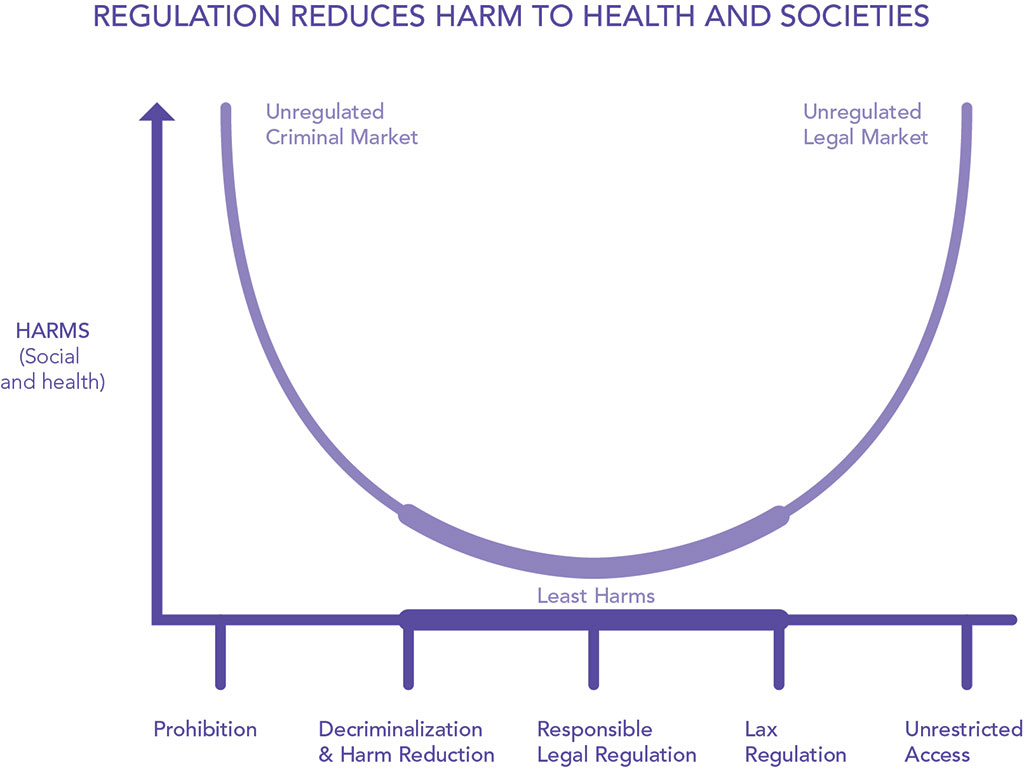
\includegraphics[width=0.57\linewidth]{figures/fig1_regulation_spectrum.jpeg}
  \caption{Expert appraisals of drug regulation place the least harmful regimes between prohibition and an unrestricted legal market \parencite{globalcommission2018}.}
  \label{fig:spectrum}
\end{figure}

LISS measured support for drug regulation in ap08a \parencites{vanbeijsterveld2008}[see also][]{vandersar2011} and gd12a \parencites{vanboekel2012}[see also][]{palali2017}. However, the questions asked provide little information on topical issues such as the closed coffeeshop-chain experiment \parencite{knottnerus2023}, the sale of tobacco in separate stores or medical prescription of MDMA \parencite{staatscommissie2024}, all of which postdate the 2008 and 2012 measurements. More recently, the Eurobarometer found 90\% support for banning heroin, cocaine and ecstasy. But \textcite{palladino2018} called for ``a more detailed questionnaire'' since that 90\% figure conceals the distinction at issue: prohibition, decriminalised use, medical supply and harm reduction all count as a ban.

How policy positions arise is the subject of attitude research \parencite[see for example][]{chambon2022}. One way to model attitudes is as networks of beliefs, feelings and behaviours \parencite[see Figure~\ref{fig:network}]{dalege2016,dalege2018}. Properties of attitudes can then be modelled as network properties, for example, attitude strength can be defined as network connectivity. Furthermore, interventions can be identified by measuring the effect an attitude component has on the rest of the network (i.e., its centrality).

\begin{figure}[H]
  \centering
  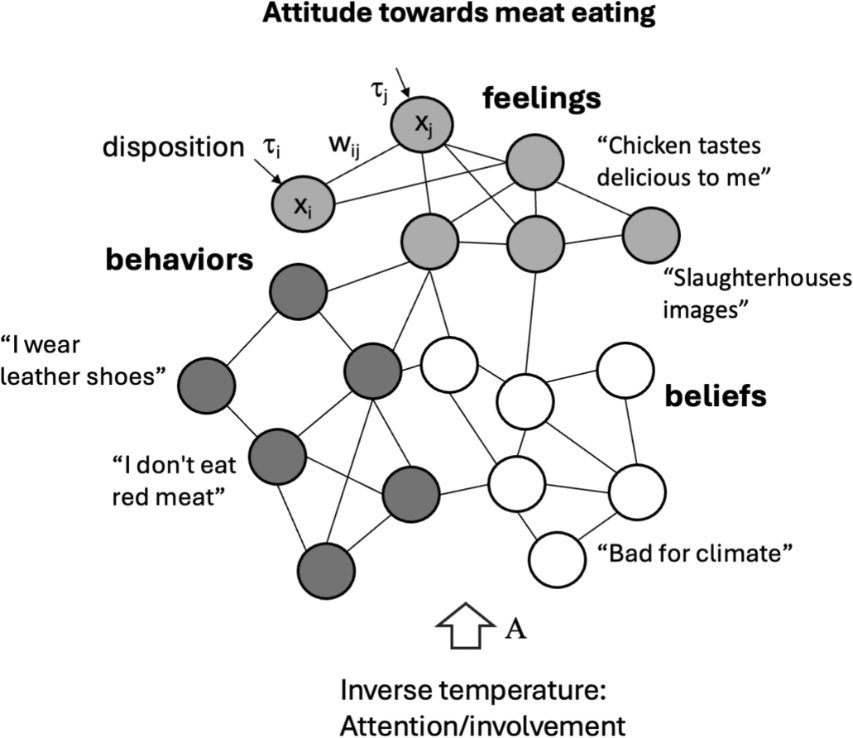
\includegraphics[width=0.6\linewidth]{figures/fig2_attitude_network.png}
  \caption{An attitude modelled as a network of beliefs, feelings and behaviours; involvement acts as the inverse temperature of the network \parencite[after][]{vandermaas2026}.}
  \label{fig:network}
\end{figure}

However, to date no instrument measures the full structure of beliefs, feelings and behaviour underlying drug regulation preferences \parencite[but see][]{greer2019,wilkins2022,hamrak2026}. Similarly, to date no instrument has been developed that measures drug policy preferences as an ordered set of regulatory models per substance. Combining the two yields support for seven regulatory models across nine substances together with the attitude dynamics behind them, usable for instance in public health campaigns.

% ---------------------------------------------------------------------------
\section{Research questions}

\textbf{Societal motivation.} We aim to map the Dutch drug regulation debate.

\textbf{RQ1.} Where does the Dutch public stand on the regulation spectrum, per substance, and what do those positions rest on? Respondents place nine substances on a 0--100 slider anchored by described policy models (see Section~\ref{sec:content} for substances and anchors). We describe the distribution per substance and explain it using the attitude items. The result is a map of the debate: which regulatory models are supported, and which beliefs, feelings and behaviours mark out the competing positions.

\textbf{Scientific motivation.} The Causal Attitude Network (CAN) model can be estimated using the binary Ising model or the ternary Blume-Capel model \parencite{dalege2016,dalege2018,vandermaas2026}. In networks with binary nodes, high involvement drives the network to one of two extremes \parencite[i.e., the attitude radicalizes,][]{vandermaas2003,vandermaas2020}. However, involved respondents frequently answer in the middle \parencite{sturgis2014,hoffstadt2025}. The ternary node extension therefore allows for a stable neutral position when involvement is high \parencite{vandermaas2026}.

The midpoint of most attitude scales is ambiguous: a middle answer cannot be told from a non-answer. Drug policy is a favourable test case: the extreme responses are the naïve options while the middle options require deliberation. We also offer a \emph{no opinion} option separately, distinguishing deliberate neutrality from ``don't know'' \parencite{sturgis2014,kankaras2025}.

\textbf{RQ2.} How does the structure of a respondent's attitude network relate to their position on the drug regulation spectrum? The ternary model predicts that cautious, involved respondents hold stable middle positions. Under the binary model an involved respondent sits at one of the extremes. We are interested in under which conditions an involved middle appears.

% ---------------------------------------------------------------------------
\section{Methodological approach}

\subsection{Samples} Two pilots studies were conducted: a convenience sample ($n = 121$) and quota sample of Dutch adults ($n = 120$). The main study consisted of a single cross-sectional wave taken through Kieskompas.

\subsection{Instrument} 

% \textbf{Policy sliders.} Respondents placed nine substances, \emph{alcohol, tabak, cannabis, psychedelica, MDMA, cocaïne/crack, speed, heroïne} and \emph{zware pijnstillers}, on a 0--100 slider anchored by nine described regulatory models:

% For developing our attitude items, we draw on \cite{saris2004}'s typology of basic concepts-by-intuition, which links the concepts measured in surveys to the linguistic structure of the assertions used to measure them. The typology distinguishes, among others, evaluations, cognitive judgments, relations, evaluative beliefs, norms and policies. Table 1 classifies each of our items accordingly. Evaluations such as "The war on drugs is a failure" have been found to be good predictors of policy stance \parencite{bergquist2022}. However, this may simply reflect their conceptual proximity to the outcome \parencite{vysevkova2026}. 

% Indeed, in our pilots, \textit{Het is verstandig om heroïne te geven aan mensen die eraan verslaafd zijn} was found to be the strongest predictor of support for legalization of hard drugs. But was removed in favour of assertions expressing support for specific interventions or consequence beliefs: \textit{Als een achtienjarige die ik goed ken XTC wil nemen, zou ik zeggen: laat de pil eerst testen.} and \textit{Als de verkoop van drugs wordt toegestaan, komen mensen met een drugsprobleem makkelijker bij de juiste hulp terecht.} \parencite{ajzen1977}.

We may start by parsing the debate into two polarised camps: the prohibitionists and the legalisers. The core difference between the prohibitionists and the legalizers is what they see as cause of the drug-related harms: prohibitionists believe drug use to be 


The core argument of the prohibitionists is traditionalist and moral. Prohibitionists view drugs as a new thing entirely. Something which emerged with globalization and should be fought back. Drug users are thus to blame for drug related crime: "Bedenk wat je doet en weet hoe ontwrichtend de drug is voor onze samenleving" (item A; \itemstats[il,r,inv]{A}; Grabberhaus in 2019, BNR). Core to this narrative is that alcohol and tabacco are not drugs (item M \itemstats[il,le,r,inv]{P}). The moral argument by prohibitionists is supported by a pragmatic belief: prohibition has a deterring effect on use (item B; \itemstats[il,r,inv]{B}). If we would all join the cause, drug use will disappear. This, they argue, is goal of drug regulation (item v; \itemstats[il,r,inv]{v}). 

The core argument of the legalisers is progressive and pragmatic. Legalisers view drugs as existing since the dawn of man. The problems, they argue, are rather a consequence of prohibition (item H; \itemstats[il,r,inv]{H}). By ending prohibition, the problems will similarly disappear. Their position is based on their conviction that people should be free to choose to take harmful substances (item O; \itemstats[il,r,inv]{O}). In the extreme, any form of interventionism is viewed as malpractice. 

However, upon closer inspection both fundamental positions are untenable.  

A principled prohibitionist must is faced with the fact that: "In an open society, drugs are quite simply available” (Els Borst; De Kort \& Cramer, 1999). A principled prohibitionist may argue that through law-and-order and prevention, supply and demand can effectively be decreased. However, not even prohibitionists seem to believe this in the efficacy of law-and-order measures (see floor and ceiling effects in figure \ref{fig:item i and ii}). Indeed, previous research has shown that instrumental rationales for punishment are rather driven mainly by retributive or symbolic concerns \parencite{carlsmith2002,tyler1982}. 

Similarly, prevention. However, it is a matter of disagreement whether said campaigns should be focused on prevention or harm reduction (item E; formerly item ix; \itemstats[il,r,inv]{ix}).

A more involved prohibitionist will thus come to recognize that some form of legal supply is necessary. And that what is necessary is a balancing act between the two. 

% The main first problem a prohibitionists must deal with is the inability of society to deal with drug-related crime. The two ways of reducing the illicit market are supply reduction and demand reduction. The latter is primarily pursued through the criminal justice system (item C;  \itemstats{ii}; note that item i was dropped due to a ceiling effect), 


The main complication for legalisers is that drugs do come with inherent risks, and that it makes sense to shield people from those risks (item N; formerly item xvi; \itemstats[il,r,inv]{xvi}, and item M; \itemstats[il,r,inv]{M}; also note that item had bivariate correlation of .56, with viii). 

A more involved legalisers will thus come to recognize that some form of restriction is necessary. And that what is necessary is a balancing act between the two. 

The second complication for prohibitionists is that rather than protecting the public, prohibition may actually be imposing excess public health harms. The most straightforward way of dealing with this concern is to simply ostracize drug users (item xiii; \itemstats[il,r,inv]{xiii}). Alternatively, they might argue that we need to offer drug abusers better health care, instead of condoning use through legalization. Counterarguments are that people are currently forced to the illicit market because their public health needs aren't met (item D) or that drug abusers can be helped better with drugs are sold legally (item F; \itemstats[il,r,inv]{F}). Most notably, the very drugs themselves may become more harmfull due to prohibition (one often cited phenomenon is the iron law of prohibition; item G; \itemstats[il,r,inv]{G}).  

The second complication for legalisers is that the the legal sale of drugs may not be sufficient reduce crime. More specifically, a balancing act between the reduction of the illicit market and the protection of public health becomes necessary. By allowing commercial parties to participate in the legal market (item K) or increasing the availability of supply (item L), the illicit market can be more effectively reduced. However both also impose excess harm on public health. 

A third complication is that countries are that international law prohibits drug regulation (item I; \itemstats[il,r,inv]{I}).

Lastly, we may differ in our aptitudes for exploring exploring the world of mind altering substances (item M \itemstats[il,le,r,inv]{M}. And some

% the need to argue for law-and-order approaches at dealing with drug-related crime (IDPC Report off track, crime citations). Interestingly, while neither prohibitionists nor legalisers seem to believe in the efficacy of a law-and-order approach (see floor and ceiling effects in figure \ref{fig:item i and ii}), both items remain excellent predictors (item i; \itemstats[il,r,inv]{i}; item ii; \itemstats{ii}). Previous research has shown that instrumental rationales for punishment are rather driven mainly by retributive or symbolic concerns \parencite{carlsmith2002,tyler1982}. Item \textit{i} was therefore dropped and \textit{ii} re-written to item C.



\begin{figure}
    \centering
    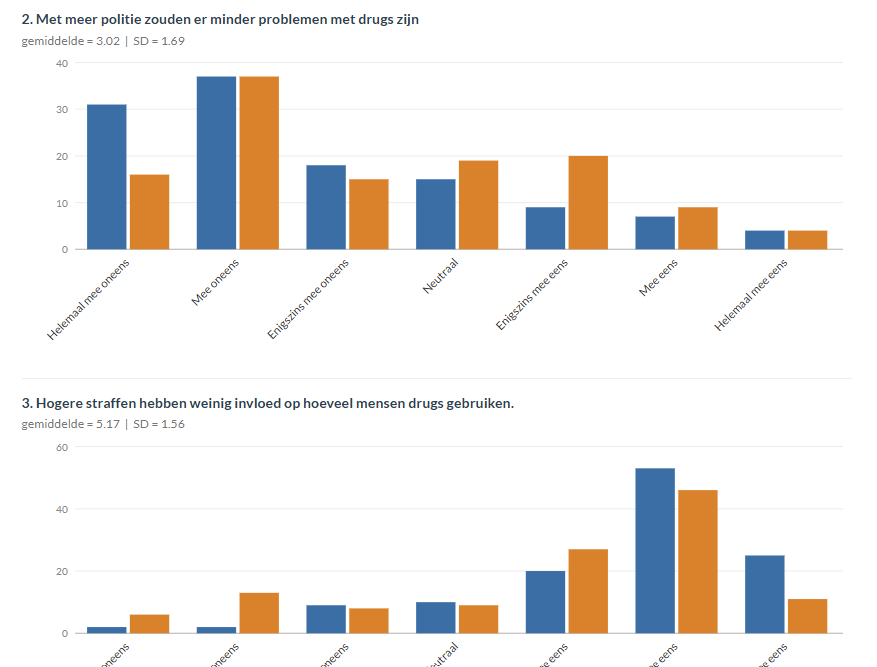
\includegraphics[width=0.5\linewidth]{image.png}
    \caption{item i, Met meer politie zouden er minder problemen met drugs zijn (b = 3.06***; item-rest = .42), and, item ii, Hogere straffen hebben weinig invloed op hoeveel mensen drugs gebruiken (b = 3.73***; item-rest = .43)}
    \label{fig:item i and ii}
\end{figure}




\begin{table}[htbp]
\centering
\small
% 1) Build the 15-item block first so its height can be measured
\sbox\itembox{%
\begin{tabular}[c]{@{}P{\wrat}P{\witem}P{\wtyp}@{}}
a) binding morals & Drugsgebruik is slecht voor de normen en waarden van onze samenleving. & Norm \\ \addlinespace[2pt]
b) deterrence effect & Als de verkoop van bepaalde drugs wordt toegestaan, zullen deze drugs meer gebruikt worden. & Relation \\ \addlinespace[2pt]
c) law-and-order & De politie moet meer tijd aan het bestrijden van het drugsprobleem & Policy \\ \addlinespace[2pt]
d) self-medication & Mensen die medicijnen illegaal kopen, doen dat omdat ze echt klachten hebben. & Relation \\ \addlinespace[2pt]
e) harm reduction & Als een achttienjarige die ik goed ken XTC wil nemen, zou ik zeggen: laat de pil eerst testen. & Action tendency \\ \addlinespace[2pt]
f) care-accessibility & Als de verkoop van drugs wordt toegestaan, komen mensen met een drugsprobleem makkelijker bij de juiste hulp terecht. & Relation \\ \addlinespace[2pt]
g) product safety & Drugsgebruik is minder gevaarlijk als de verkoop wordt toegestaan. & Relation \\ \addlinespace[2pt]
h) organised crime & Er zou in Nederland minder criminaliteit zijn als de verkoop van drugs wordt toegestaan. & Relation \\ \addlinespace[2pt]
i) international & We krijgen problemen met andere landen, als Nederland de verkoop van drugs toestaat. & Evaluative belief \\ \addlinespace[2pt]
j) curiosity & Als iemand een drug heeft gebruikt die ik niet ken, zou ik ernaar vragen. & Action tendency \\ \addlinespace[2pt]
k) commercialisation & Winkels die winst mogen maken, houden mensen beter weg bij de dealer dan winkels zonder winst. & Evaluative belief \\ \addlinespace[2pt]
l) availability & Hoeveel winkels alcohol verkopen, maakt niet uit voor hoeveel mensen drinken. & Relation \\ \addlinespace[2pt]
m) normalisation & Jongeren komen makkelijker aan drugs als de verkoop wordt toegestaan. & Relation \\ \addlinespace[2pt]
n) risk-taking & Ik neem weleens een drankje of drug aan van iemand die ik niet goed ken. & Behaviour \\ \addlinespace[2pt]
o) individualising morals & Mensen mogen zelf beslissen of ze ongezonde middelen gebruiken. & Norm
\end{tabular}}%
\setlength\itemheight{\dimexpr\ht\itembox+\dp\itembox\relax}%
% 2) Outer table: the policy column gets exactly that height
\begin{tabular}{@{}P{\wpol}P{\wrat}P{\witem}P{\wtyp}@{}}
\toprule
\textbf{Policy} & \textbf{Rationale} & \textbf{Item} & \textbf{Type} \\
\midrule
\parbox[c][\itemheight][s]{\wpol}{\raggedright
  \pol{Verbod}                                \hrule
  \pol{Alleen voor onderzoek}                 \hrule
  \pol{Alleen als behandeling}                \hrule
  \pol{Alleen op recept}                      \hrule
  \pol{Alleen in speciaalzaak, zonder winst}  \hrule
  \pol{Alleen in speciaalzaak, met winst}     \hrule
  \pol{Overal te koop, zonder reclame}        \hrule
  \pol{Overal te koop, met reclame}           \hrule
  \pol{Vrije verkoop}}
  & \multicolumn{3}{l@{}}{\usebox\itembox} \\
\midrule
 & p) double standard & Verboden harddrugs zijn ongezonder dan alcohol en tabak. & Judgment \\
\bottomrule
\end{tabular}
\end{table}


\begin{table}[ht]
\centering\small
\caption{Pilot statistics of the items in the item table (new items have none).}
\label{tab:items}
\begin{tabular}{l>{\raggedright\arraybackslash}p{7.5cm}rrrr}
\toprule
& Item & item-rest & $b_{\mathit{il}}$ & $b_{\mathit{le}}$ & $r_{\mathit{inv}}$ \\
\midrule
A) & \itemtext{A} & \rrest{A} & \bil{A} & \ble{A} & \rinv{A} \\
B) & \itemtext{B} & \rrest{B} & \bil{B} & \ble{B} & \rinv{B} \\
C) & \itemtext{C} & \rrest{C} & \bil{C} & \ble{C} & \rinv{C} \\
D) & \itemtext{D} & \rrest{D} & \bil{D} & \ble{D} & \rinv{D} \\
E) & \itemtext{E} & \rrest{E} & \bil{E} & \ble{E} & \rinv{E} \\
F) & \itemtext{F} & \rrest{F} & \bil{F} & \ble{F} & \rinv{F} \\
G) & \itemtext{G} & \rrest{G} & \bil{G} & \ble{G} & \rinv{G} \\
H) & \itemtext{H} & \rrest{H} & \bil{H} & \ble{H} & \rinv{H} \\
I) & \itemtext{I} & \rrest{I} & \bil{I} & \ble{I} & \rinv{I} \\
J) & \itemtext{J} & \rrest{J} & \bil{J} & \ble{J} & \rinv{J} \\
K) & \itemtext{K} & \rrest{K} & \bil{K} & \ble{K} & \rinv{K} \\
L) & \itemtext{L} & \rrest{L} & \bil{L} & \ble{L} & \rinv{L} \\
M) & \itemtext{M} & \rrest{M} & \bil{M} & \ble{M} & \rinv{M} \\
N) & \itemtext{N} & \rrest{N} & \bil{N} & \ble{N} & \rinv{N} \\
O) & \itemtext{O} & \rrest{O} & \bil{O} & \ble{O} & \rinv{O} \\
P) & \itemtext{P} & \rrest{P} & \bil{P} & \ble{P} & \rinv{P} \\
\bottomrule
\end{tabular}
\end{table}


\begin{table}[ht]
\centering\small
\caption{Pilot items not retained in the item table.}
\label{tab:dropped-items}
\begin{tabular}{l>{\raggedright\arraybackslash}p{7.5cm}rrrr}
\toprule
& Item & item-rest & $b_{\mathit{il}}$ & $b_{\mathit{le}}$ & $r_{\mathit{inv}}$ \\
\midrule
\textit{i}) & \itemtext{i} & \rrest{i} & \bil{i} & \ble{i} & \rinv{i} \\
% ceilling effect

\textit{ii}) & \itemtext{ii} & \rrest{ii} & \bil{ii} & \ble{ii} & \rinv{ii} \\
% is nu B 

\textit{iii}) & \itemtext{iii} & \rrest{iii} & \bil{iii} & \ble{iii} & \rinv{iii} \\
% voorspelt alleen cannabis goed (soft-hard drugs onderscheid in algemeen is dit waar voor) 

\textit{iv}) & \itemtext{iv} & \rrest{iv} & \bil{iv} & \ble{iv} & \rinv{iv} \\
% veel midden responses

\textit{v}) & \itemtext{v} & \rrest{v} & \bil{v} & \ble{v} & \rinv{v} \\
% maybe not that bad

\textit{vi}) & \itemtext{vi} & \rrest{vi} & \bil{vi} & \ble{vi} & \rinv{vi} \\

\textit{vii}) & \itemtext{vii} & \rrest{vii} & \bil{vii} & \ble{vii} & \rinv{vii} \\
\textit{viii}) & \itemtext{viii} & \rrest{viii} & \bil{viii} & \ble{viii} & \rinv{viii} \\

\textit{ix}) & \itemtext{ix} & \rrest{ix} & \bil{ix} & \ble{ix} & \rinv{ix} \\
% zit nu in schaal

\textit{x}) & \itemtext{x} & \rrest{x} & \bil{x} & \ble{x} & \rinv{x} \\
% hoge bivariate correlation between dubbele maat item. 

\textit{xi}) & \itemtext{xi} & \rrest{xi} & \bil{xi} & \ble{xi} & \rinv{xi} \\
\textit{xii}) & \itemtext{xii} & \rrest{xii} & \bil{xii} & \ble{xii} & \rinv{xii} \\
% moet terug

\textit{xiii}) & \itemtext{xiii} & \rrest{xiii} & \bil{xiii} & \ble{xiii} & \rinv{xiii} \\
\textit{xiv}) & \itemtext{xiv} & \rrest{xiv} & \bil{xiv} & \ble{xiv} & \rinv{xiv} \\
\textit{xv}) & \itemtext{xv} & \rrest{xv} & \bil{xv} & \ble{xv} & \rinv{xv} \\
\textit{xvi}) & \itemtext{xvi} & \rrest{xvi} & \bil{xvi} & \ble{xvi} & \rinv{xvi} \\
% is nu N

\textit{xvii}) & \itemtext{xvii} & \rrest{xvii} & \bil{xvii} & \ble{xvii} & \rinv{xvii} \\
\textit{xviii}) & \itemtext{xviii} & \rrest{xviii} & \bil{xviii} & \ble{xviii} & \rinv{xviii} \\
\bottomrule
\end{tabular}
\end{table}


d) Mensen die medicijnen illegaal kopen, doen dat vaak omdat de doktor het niet voorschrijft.
f) Mensen met een drugsprobleem makkelijker worden beter geholpen als de verkoop van drugs wordt toegestaan.
k) Mensen willen geen drugs kopen bij de overheid.
l) Hoeveel mensen een middel gebruiken, hangt meer af van cultuur dan van het aantal winkels dat het verkoopt.


Als de verkoop van drugs wordt toegestaan, zullen vooral kwetsbare mensen de nadelen ervaren. 

\textbf{Repeated LISS items (5).} The items from ap08a and gd12a mentioned above, in their original wording and scale, for trend comparison.

\textbf{Background.} Taken from the LISS background variables; vote intention taken from the Politics and Values core study (cv) rather than asked in-survey.


In the pilot data the attitude items already explained a substantial share of slider variance (adjusted $R^2$ between .27 and .42 across substances). Item screening followed the reporting standards for cross-sectional network analysis: item redundancy based on $\rho$, leave-one-out $\Delta R^2$, and corrected item-rest \parencite{burger2022,chambon2026}. Wording is at B1 Dutch level. Own-use items are anonymous and skippable. The survey closes with a referral to the Drugs Infolijn.

\textbf{Analysis.} RQ1 is descriptive and exploratory. Per substance the location, dispersion and modality will be reported. The policy sliders are regressed on the attitude items. RQ2 uses a mixed graphical model, estimated with EBIC model selection \parencite{haslbeck2020}, with bootstrapped edge accuracy and centrality stability \parencite{epskamp2018}. Involvement enters as continuous moderator of edge weights \parencite{haslbeck2021}. Modality is estimated per involvement quartile \parencite{hoffstadt2026}.

% ---------------------------------------------------------------------------
\section{Implications for research, practice and/or society}

\textbf{For research.} This study can progress attitude theory by improving our understanding of deliberated neutrality, and by adjudicating between binary and ternary node models on population data.

\textbf{For survey practice.} Surveys typically offer a middle option and treat it as indicating no opinion. Evidence that the middle option in policy questions can represent deliberate neutrality, and the conditions under which this occurs, is relevant wherever the middle of a policy scale is itself a policy. This study's results may thus bear on how to interpret past and design future LISS studies.

\textbf{For Dutch society.} Attitudes towards the regulation of psychoactive substances seem to be changing in the West \parencite{felson2019,gallup2023}. Regulatory models which were unthinkable decades ago are now in place: commercial legalization of cannabis in many US states and a ban on tobacco sales to anybody born after 2008 in the UK \parencite{tobaccovapesact2026}. As described above, the public is usually consulted in impoverished terms. And government communication is sometimes counterproductive \parencite[e.g., messaging that presents drug use as normalised may increase use,][]{vanwingerde2023}. How we discuss drug regulation matters: in an Irish citizens' assembly 85\% rejected the status quo, 58.6\% chose a hybrid of different approaches for different drugs, and no universal option drew more than 18.4\% \parencite{citizensassembly2024}. Drug regulation requires steady deliberation and incremental steps \parencite{maccoun2001}.

Our measurement is usable by the \emph{Ministerie van Volksgezondheid, Welzijn en Sport} \parencite{kamerstukken573} and the \emph{Ministerie van Justitie en Veiligheid} \parencite{kamerstukken572}, and by the municipalities running the closed coffeeshop-chain experiment. Finally by LISS conducting this survey, the spectrum can be linked to the 2008 and 2012 LISS items.

% ---------------------------------------------------------------------------

\section{discussion}

- we are missing arguments in favour of commercialisation, beyond competing with the illicit market. In other words, why don't people want to go to government stores for alcohol? Out of laziness? Distrust of the government? 

% ---------------------------------------------------------------------------
% Listed in the original reference list but not cited in the text:
\nocite{goode2004,vangelder2024}
\printbibliography

% ---------------------------------------------------------------------------
\clearpage
\appendix


\end{document}
